\section{Внутренняя мотивация}\label{subsec:intrinsic_motivation}

\subsection{Вспомогательные задачи}

В обучении с подкреплением типична ситуация разреженной функции награды, когда агенту редко поступает сигнал от среды. Например, в худшем случае функция награды представляет собой константу, имеющую смысл <<штрафа за потерю времени>>, а в конце эпизода нам приходит условно +1, если задача была успешно решена.  

\begin{definition}
Задачей \emph{поиска} будем называть задачу со следующей функцией награды:
\begin{equation}\label{searchreward}
r(s, a) = \begin{cases}
+1 \quad & s \in \St^+ \\
\const \quad & s \not\in \St^+ \\
\end{cases}    
\end{equation}
где $\St^+$ --- множество терминальных состояний, $\const \le 0$ --- штраф за потерю времени.
\end{definition}

Задача поиска сложна тем, что сигнала от среды нет. Пока мы не решим задачу, оптимизируемый функционал представляет собой плато, а наши RL алгоритмы, как и любые методы оптимизации, работают за счёт разницы в сигнале.

Что в таких ситуациях делать? Первая возможность --- учить модель динамики среды, если она неизвестна. Найти сигнал от среды это скорее всего не поможет, поскольку экспоненциальный перебор всевозможных будущих траекторий не сильно лучше случайного блуждания в среде.

Мы придумаем себе другую, вспомогательную задачу, которую мы сможем решать в \emph{self-supervised} режиме --- режиме, не требующем никакого сигнала от среды, никакой <<разметки>>.

\begin{definition}
Для данной среды $(\St, \A, \Trans)$ \emph{вспомогательной задачей} называется задача обучения с подкреплением для MDP $(\St, \A, \Trans, r^{\intr})$, где $r^{\intr}$ --- \emph{внутренняя мотивация} (intrinsic motivation) или \emph{внутренняя награда} (intrinsic reward function), определяемая самим агентом.
\end{definition}

Слова <<определяемая самим агентом>> означает, что эта функция нам не дана. Исходная задача, которую мы хотим решить, состоит в оптимизации в данной среде некоторой \emph{внешней функцией награды} (extrinsic reward function) $r^{\extr}$, также называемой \emph{внешней мотивацией} (extrinsic motivation). Однако, если эта функция награды, например, для задачи поиска \eqref{searchreward} и всегда константна, то нам необходимо откуда-то взять какой-то другой обучающий сигнал. Этот сигнал нам придётся придумать <<самим себе>>, при помощи нового модуля в обучающейся системе.

Какой обучающий сигнал мы хотим получить? Во-первых, плотный, чтобы было, на чём обучаться базовому алгоритму. Во-вторых, осмысленный: награждающий за развитие каких-то <<полезных>> в среде навыков, которые могут пригодиться для взаимодействия, условно, вне зависимости от того, какой на самом деле окажется та внешне мотивированная задача, которую агент призван решать.

\begin{example}
Идея, можно сказать, вдохновлена подобной <<внутренней наградой>> человека, поощряющей такое поведение, как игра, любопытство, стремление к познанию. В ходе игрового поведения, человек улучшает своё представление о том, как работает мир вокруг него, по каким законам он устроен и как он своими действиями может влиять на будущее состояние мира и вызывать те или иные явления. Такое более интеллектуальное <<самообучение>> не только ускоряет поиск сигнала от среды, но и позволяет агенту выработать широкий набор умений, которые скорее всего окажутся полезны для достижения заданной внешней наградой цели, какой бы она ни оказалась.
\end{example}

Придумать в общем случае такой сигнал непросто, и могут возникать ситуации, когда внутренняя мотивация <<промотивирует>> агента <<залипнуть>> в какой-то области среды.

\begin{definition}
Проблемой \emph{прокрастинации} (procrastination) называется ситуация, когда в некоторой области в среде внутренняя мотивация выдаёт высокий (и не снижающийся с течением обучения) сигнал, перебивающий остальные мотивации агента.
\end{definition}

\subsection{Совмещение мотиваций}

По умолчанию всегда считается, что внешняя и внутренняя мотивация складываются:
\begin{equation}\label{sumgoal}
r(s, a) \coloneqq r^{\extr}(s, a) + \alpha r^{\intr}(s, a),
\end{equation}
где $\alpha$ --- масштабирующий гиперпараметр. Для простоты далее будем считать $\alpha \HM= 1$.

Заданная так награду можно оптимизировать любым <<базовым>> алгоритмом RL, ничего не подозревающим о разложении. Но понятно, что агенту доступно каждое слагаемое по отдельности (коли внешняя награда выдаётся средой, а внутренняя генерируется внутри самого алгоритма); как мы можем это использовать?

Пусть оценочные функции с индексом $\extr$ соответствуют оценочным функциям для внешней мотивации, с индексом $\intr$ --- внутренней мотивации, без индекса --- суммарной мотивации. Тогда:
\begin{proposition}
\begin{equation}\label{valuefunctionssum}
\begin{aligned}
Q^\pi(s, a) &= Q^\pi_{\extr}(s, a) + Q^\pi_{\intr}(s, a) \\
V^\pi(s) &= V^\pi_{\extr}(s) + V^\pi_{\intr}(s)
\end{aligned}
\end{equation}
\begin{proof}
По определению.
\end{proof}
\end{proposition}

\begin{proposition}
В общем случае аналогичное разложение для $Q^*, V^*$ неверно.
\begin{proof}
Максимум суммы может быть меньше суммы максимумов. Действительно, пусть первое действие даёт внешнюю +1, а второе действие даёт внутреннюю +1 (иначе по нулям); тогда оптимальные оценочные функции равны $V^*_{\intr}(s) = V^*_{\extr}(s) = +1$, но оптимальная V-функция для суммы наград равна не 2, а 1, поскольку выбрать одновременно два действия нельзя и между мотивациями придётся выбирать.
\end{proof}
\end{proposition}

\begin{proposition}
В общем случае аналогичное разложение для $\Z^\pi$ неверно.
\begin{proof}
Это связано с тем, что внутренняя и внешняя мотивация могут быть скоррелированы, и этой информации при доступе к отдельным $\Z^\pi_{\extr}$ и $\Z^\pi_{\intr}$ у нас нет. Действительно: пусть известно, что для некоторых $s, a$ с вероятностью 0.5 $\Z^\pi_{\extr}(s, a)$ принимает значение +1, а иначе 0, и тоже самое для $\Z^\pi_{\intr}(s, a)$. Мы могли бы сказать, что распределение суммы $\Z^\pi_{\extr}(s, a) + \Z^\pi_{\intr}(s, a)$ имеет такой вид: с вероятностью 0.25 мы получим +2, с вероятностью 0.5 получим +1, и с вероятностью 0.25 не получим ничего. Однако, тогда мы предполагаем независимость этих случайных величин, а это может быть неправдой: например, вдруг мы получаем внешнюю +1 тогда и только тогда, когда получаем внутреннюю +1. Тогда $\Z^\pi(s, a)$ суммы мотиваций есть на самом деле +2 с вероятностью 0.5 и +0 иначе.
\end{proof}
\end{proposition}

\begin{proposition}
В общем случае аналогичное разложение для $\Z^*$ неверно.
\end{proposition}

\needspace{5\baselineskip}
\begin{wrapfigure}{r}{0.35\textwidth}
%\vspace{-0.4cm}
\centering
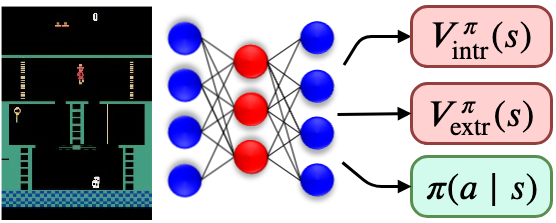
\includegraphics[width=0.35\textwidth]{Images/sepheads.png}
%\vspace{-0.5cm}
\end{wrapfigure}

Итак, в алгоритмах на основе Policy Gradient и Policy Iteration подходов можно учить оценочные функции каждого слагаемого в награде по отдельности.
%Для каждой мотивации у моделей оценочных функций заводится своя голова, которая учится на свой сигнал; далее, при обучении актёра используется сумма этих выходов.

\begin{remark}
Этим фактом можно также пользоваться в ситуациях, когда награда представлена в виде суммы нескольких слагаемых (очень типичная ситуация), и агенту доступно полное разложение на эти слагаемые. Это позволит по ходу оптимизационного процесса <<включать>> и <<отключать>> мотивации, что бывает очень удобно.
\end{remark}

\begin{remark}
Разложение также позволяет использовать для разных мотиваций разные коэффициенты дисконтирования, а также сделать внутреннюю мотивацию неэпизодичной, чтобы агент мог осознанно провести ресет среды в ходе взаимодействия и <<вернуться в начало для совершения ещё одной попытки>>.
\end{remark}

Разложение также позволяет во внутренней мотивации игнорировать понятия эпизодов: это означает, что агент рассматривает весь процесс решения вспомогательной задачи как один большой никогда не заканчивающийся эпизод, не используя флаги $\done$ из среды. Такой агент учитывает, что если он окажется в терминальном состоянии, то произойдёт сброс среды, и он окажется в стартовом состоянии $s_0 \HM\sim p(s_0)$, для которого значение $V^{\intr}(s)$ может быть высоким. Это может мотивировать агента прерывать текущий <<неудачный>> эпизод ради того, чтобы начать новый, что иногда может быть полезно.

\vspace{0.2cm}
\begin{example}[Агент в яме]
В среде существует некоторая труднодоступная область, которую агент внутренне мотивирован посетить. Агент предпринимает попытку добраться до области, но падает в яму. Оценочная функция для внешней мотивации знает, что из ямы уже не выбраться, и оценивает действие <<закончить эпизод>> как негативное (<<смерть>>), остальные действия как безрезультатные (+0). Оценочной функции для внутренней мотивации, допустим, известно, что из ямы уже не выбраться, и, в случае, если она обучается эпизодично, оценивает любые действия как безрезультатные (+0). Если же оценочная функция игнорирует понятие эпизодов, агент знает, что он может произвести сброс среды и, в частности, попробовать ещё раз добраться до труднодоступной области. Это может промотивировать агента не сидеть в яме, оттягивая негативный, но неизбежный эффект смерти, а приступить к следующему эпизоду обучения.
\end{example}

\subsection{Exploration Bonuses}

Как строить $r^{\intr}$? Что должен делать агент, который попал в среду, и не получает никакого внешнего сигнала? На этот вопрос можно ответить по-разному.

\begin{exampleBox}[label=ex:chaosminimization]{Минимизация хаоса (chaos minimization)}
Нужно искать наиболее <<безопасные>>, стабильные области пространства состояний, где будущее наиболее предсказуемо, <<избегать сюрпризов>>. Интуицией в такой вспомогательной задаче является идея о том, что многие изобретения человечества были созданы для защиты от сюрпризов, которые, зачастую, неприятны. Существуют среды, например, тетрис, где задача <<минимизации хаоса>> коррелирует с задачей самой игры; агент, решающий такую вспомогательную задачу без доступа к внешней функции награды, <<неявно>> решает исходную задачу.
\end{exampleBox}

Мы далее рассмотрим другой ответ --- заниматься исследованием. Отчасти эта задача полностью противоположна минимизации хаоса: однако задачи не противоречат друг другу, ведь чтобы найти самую <<спокойную>> область среды и научиться до неё добираться, агенту потребуется заняться исследованием окружения и поиском этих самых стабильных областей. В этом смысле, задача исследования, вероятно, является наиболее универсальной вспомогательной задачей, которую агент может себе поставить в среде.

Мы постоянно встречались с дилеммой исследования-использования по ходу пьесы, однако теперь, когда оптимизировать внешний сигнал у нас не получается ввиду его отсутствия, <<использовать>> нам абсолютно нечего, и дилемма не стоит. Итак, считаем, что нам дана среда и есть задача <<заисследовать её>>. Как формализовать такую задачу в терминах награды?

\needspace{5\baselineskip}
\begin{wrapfigure}{r}{0.3\textwidth}
\vspace{-0.4cm}
\centering
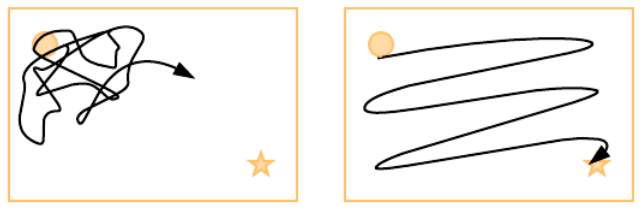
\includegraphics[width=0.3\textwidth]{Images/exploration.png}
\vspace{-0.5cm}
\end{wrapfigure}

Понятно, что случайная стратегия, которой мы часто пользовались до этого для <<исследований>>, является теоретическим решением (например, с точки зрения теоремы \ref{th:TDconvergencetheorem}). Но интуитивно, куда более оптимальным поведением является некий интеллектуальный перебор состояний в среде.

Мы уже встречались с \emph{исследовательскими бонусами} (exploration bonus) в контексте UCB-бандитов (раздел \ref{subsec:ucb}): там мы добавляли к нашей оценке Q-функции некоторое слагаемое, имевшее смысл <<награды за то, что действие редко пробовалось в прошлом>>. Наша внутренняя мотивация тоже есть такая добавка, только теперь она должна оценивать новизну посещаемых областей в среде.

Попробуем исходить из схожих соображений: будем награждать агента за посещения тех состояний, в которых он был редко. Мы можем это сделать двумя способами.

\begin{definition}
Пусть $h(s) \colon \St \to \{0, 1 \dots N\}$ --- некоторая хэш-функция состояний, называемая \emph{оракулом} (oracle), и $n(i)$ --- счётчик, сколько раз за время всего обучения нам встретились состояния с хэшем $i$. Тогда
$$r_{\intr}(s, a) \coloneqq \frac{1}{n(h(s))}$$
называется \emph{нестационарным} исследовательским бонусом; награда
$$r_{\intr}(s_t, a_t) \coloneqq \mathbb{I}[\forall t' < t \colon s_t \neq s_{t'}],$$
то есть награждение +1, если мы попали в состояние, хэш для которого $h(s_t)$ не встречался до этого в течение данного эпизода, называется \emph{эпизодичным} исследовательским бонусом.
\end{definition}

Нестационарные исследовательские бонусы затухают с ходом обучения; в пределе мы, надеемся, посетим все состояния достаточное число раз, внутренняя мотивация затухнет и мы переключимся на внешнюю мотивацию. Плохо это тем, что такая мотивация нарушает стационарность формализма MDP, так как с ходом обучения меняются счётчики посещения. Это довольно типично, что внутренняя мотивация нестационарна: модуль внутренней мотивации принципиально есть часть обучающейся системы, и он тоже постепенно <<обучается>>, следовательно, меняется. Для нас это значит, что нужно будет использовать on-policy алгоритмы для обучения на такой сигнал.

Эпизодичные бонусы, конечно же, можно считать модификацией функции награды, и поэтому подобные оракулы можно считать <<ручными эвристиками>>. Агент в том числе по итогам обучения научится в ходе одного эпизода <<бегать по всему MDP>>. Это, однако, вполне может быть полезно в каких-нибудь лабиринтах или задачах, где агенту нужно что-то где-то найти в течение самой игры. Проблема эпизодичных бонусов в том, что они формально нарушают предположение о полной наблюдаемости пространства состояний: функция награды зависит от всей прошлой истории посещения состояний в течение эпизода, и нам по-хорошему нужно переходить в формализм PoMDP.

\begin{exampleBox}[righthand ratio=0.25, sidebyside, sidebyside align=center, lower separated=false]{}
В табличных MDP, где $|\St| < +\infty$, хэш-функция по сути не нужна: $h(s) = s$. В ряде сред подобный оракул можно придумать эвристически; например, если у агента есть понятие <<координат>>, можно разделить пространство сеточкой, то есть поделив его на условные блоки, и награждать агента за <<посещение большого числа блоков>>. 

\tcblower
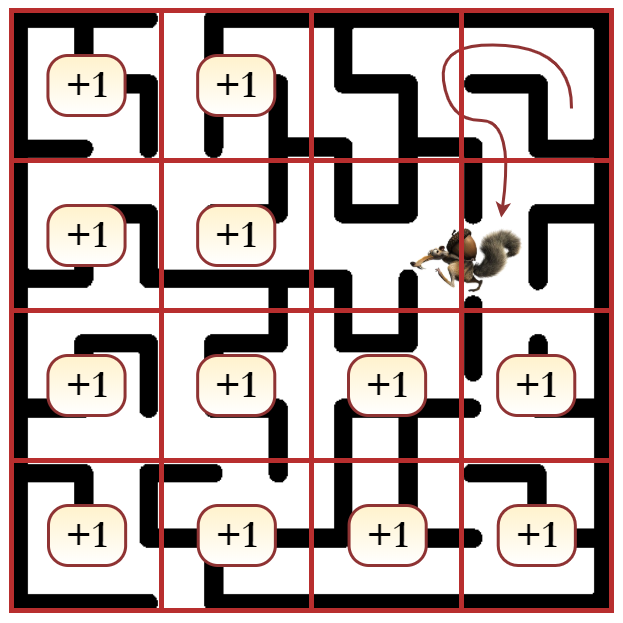
\includegraphics[width=\textwidth]{Images/maze.png}
\end{exampleBox}

\subsection{Дистилляция случайной сетки (RND)}

\needspace{5\baselineskip}
\begin{wrapfigure}{r}{0.55\textwidth}
\vspace{-0.4cm}
\centering
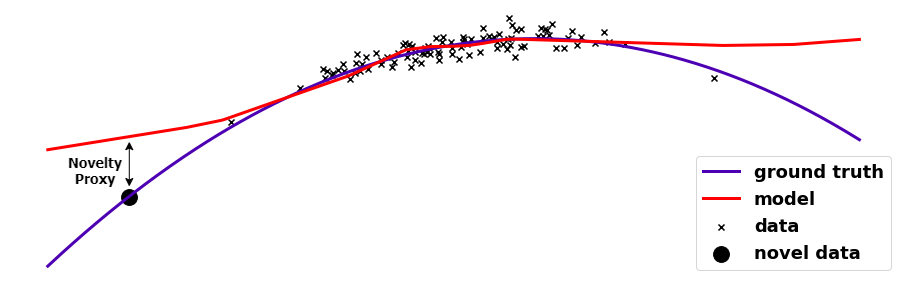
\includegraphics[width=0.55\textwidth]{Images/novelty4.png}
\vspace{-0.5cm}
\end{wrapfigure}

Понятно, что в общем случае хэш-функцию придумать сложно, и нам нужен какой-то более универсальный способ оценки новизны. Мы воспользуемся трюком из машинного обучения: известно, что если некоторая модель обучалась решать задачу регрессии, то на входных данных, не похожих на примеры из обучающей выборки, ошибка её прогнозов будет больше. Отличие предсказания модели от истинного значения целевой переменной может быть использовано как приближение \emph{оценки новизны} (novelty esimation) или \emph{аномальности} данных.

Давайте возьмём какую-нибудь случайную задачу регрессии с состояниями в качестве входов. Нам важно лишь, что значение целевой переменной должно определяться по входному состоянию детерминировано и стационарно: ведь если таргет не детерминирован, то ошибка предсказывающей модели для состояния $s$ будет (если, например, модель обучается на минимизацию MSE) в среднем равна дисперсии. В такой ситуации сигнал внутренней мотивации будет выше в тех областях пространства состояний, где дисперсия целевой переменной выше. Нестационарность, очевидно, нарушает идею подхода, поскольку ошибка модели будет связана с изменением целевой переменной, а не новизной входного состояния. 

Пусть $\phi \colon \St \to \R^d$ --- некоторая функция, строящая эмбеддинги для состояний; например, \emph{случайная сеть} (random network) --- нейросеть со случайно инициализированными весами, которые не обучаются и никак не изменяются. Пусть $f \colon \St \to \R^d$ учится предсказывать выход $\phi$, используя в качестве обучающей выборки её значения на встречавшихся в ходе обучения состояниях.

\begin{definition}
Задача обучения одной нейросети $f$ на входах-выходах другой (заданной, фиксированной) нейросети $\phi$
$$\E_s \|f(s) - \phi(s)\|_2^2 \to \min_{f},$$
где мат.ожидание $\E_s$ берётся по произвольному буферу, называется \emph{дистилляцией} (distillation).
\end{definition}

Коли ошибка выше там, где новее состояния, мы можем использовать это значение в качестве обучающего сигнала:
$$r^{\intr}(s) \coloneqq \|f(s) - \phi(s)\|_2^2$$
Интуиция понятна: если мы <<впервые>> увидели состояние $s$, модель $f$ ещё ни разу не видела, какой эмбеддинг выдаёт на нём наша случайная сеть $\phi$, и поэтому скорее всего ошибётся. Такой сигнал будет мотивировать агента отправиться в ту область среды, где обучающаяся нейросеть плохо предсказывает выход случайно проинициализированной нейросети.

\begin{remark}
Здесь и в аналогичных местах далее использование MSE не принципиально (можно использовать любую функцию потерь для регрессии). В частности, можно одну метрику использовать для функции потерь, и другую --- для расчёта внутренней мотивации.
\end{remark}

% \needspace{5\baselineskip}
% \begin{wrapfigure}{l}{0.5\textwidth}
% \vspace{-0.4cm}
% \centering
% 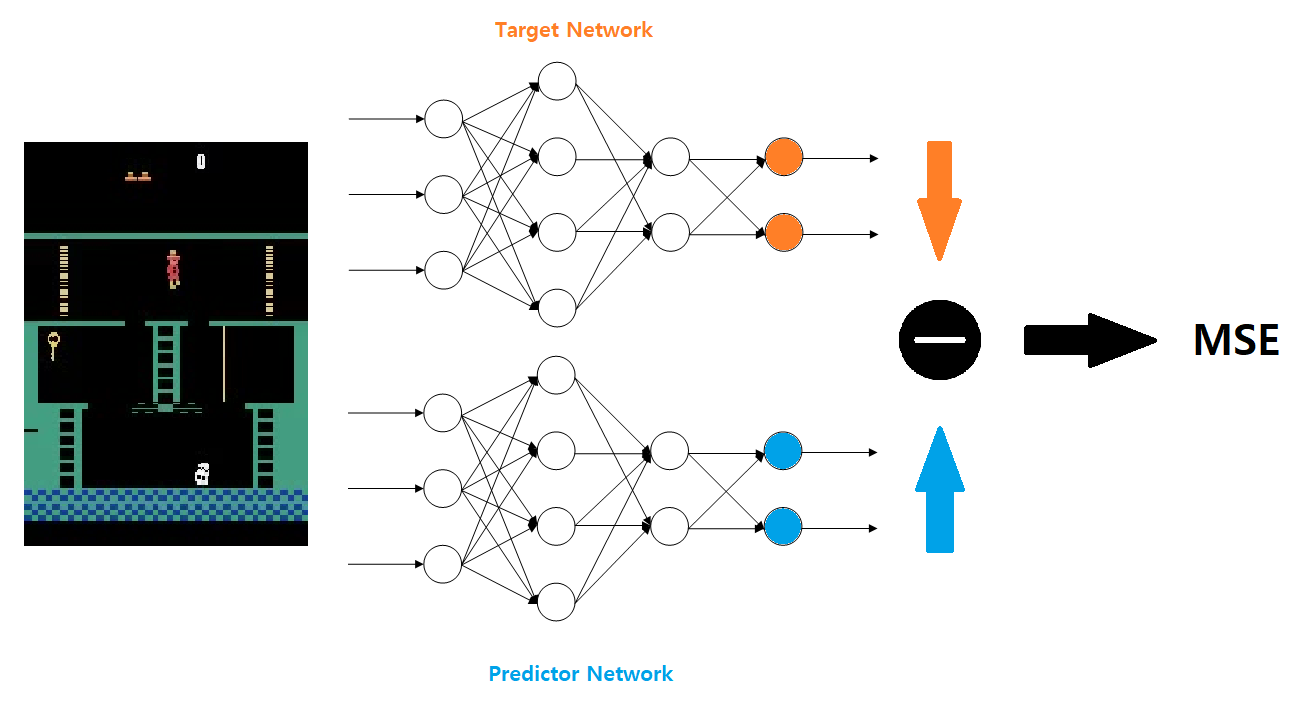
\includegraphics[width=0.5\textwidth]{Images/RND.png}
% \vspace{-0.5cm}
% \end{wrapfigure}

\begin{remark}
Авторы также предложили нормировать сигнал внутренней мотивации на его бегущее среднее отклонение, то есть <<в среднем>> выдавать некоторую константу. Это существенно упрощает масштабирование внутренней мотивации относительно внешней, но тогда <<исследование>> не будет естественно затухать с ходом обучения.
\end{remark}

\subsection{Любопытство}

\begin{definition}
\emph{Любопытством} (curiosity) называется ошибка модели мира агента.
\end{definition}

Ошибка свидетельствует о том, что агент не всё знает о той области пространства состояний, в которой был произведён неверный прогноз. Использование любопытства как внутренней мотивации приводит к тому, что агент стремится в те области среды, которые ему <<непонятны>>, в частности те, которые для агента новы, и <<дообучить>> своё представление о мире. Зачастую выбор действий, максимизирующих ошибку модели мира приводит к \emph{возникновению игрового поведения} (emergence of playing behavior), когда агент <<играет>> с доступными для взаимодействия предметами.

Любопытство и построение внутренней мотивации на основе новизны состояний немного различаются. То, что состояние ново, не означает, что оно <<незаисследовано>>, что мы ничего о нём не знаем; мы вполне можем обобщиться за счёт прошлого опыта и спокойно ориентироваться даже в том состоянии, которое технически увидели впервые.

\begin{example}[Бесконечные двери]
В ряд стоит бесконечное количество одинаковых дверей, за каждой из которых ничего нет. Агенту доступен на вход, помимо прочего, номер двери. Сигнал, построенный на основе оценки новизны состояний, будет поощрять обнаружение новых дверей, поскольку
их номер <<нов>> по сравнению со старыми. Любопытство же через некоторое время научится предсказывать, что при движении вдоль ряда агенту будут встречаться точно такие же двери, как и раньше, и что за дверьми ничего нет; сигнал затухнет. При этом, любопытство среагирует на любое изменение в описании двери, или если за очередной дверью окажется что-то непредсказуемое.

\begin{center}
    
\includegraphics[width=0.7\textwidth]{Images/doors.jpg}
\end{center}

На самом деле, разница достаточно условна: предполагается, что модель предсказания будущего способна «обобщаться» на новые состояния, что, в целом, может оказаться верным и для модели оценки новизны. Так, в приведённом примере модель оценки новизны также может перестать оценивать увеличение номера двери как «новые» состояния, и тогда поведение этих двух видов внутренней мотивации станет схожим.

% Допустим, состояние описывается натуральным числом (<<стена>>). После выбора единственного действия состояние увеличивается на единичку (<<снова стена>>). С точки зрения новизны, каждое следующее состояние --- новое. Однако, в какой-то момент мы можем понять, что следующее состояние будет на единичку больше, чем предыдущее; другими словами, мы благодаря накопленному опыту можем <<обобщиться>> и, несмотря на новизну состояния, всё равно понимать, как среда в этой области работает. Имеет ли смысл в таких ситуациях выдавать высокий сигнал внутренней мотивации?
\end{example}

Пусть внутри агента строится модель прямой динамики:
$$\E_{s,a,s'} \|f(s, a) - s'\|^2_2 \to \min_f$$
Тогда во время очередного обучающего эпизода ошибка модели $f$ на каждом шаге может рассматриваться как любопытство и задавать внутреннюю мотивацию агента:
\begin{equation}\label{curiosity}
r^{\intr}(s, a, s') \coloneqq \|f(s, a) - s'\|^2_2
\end{equation}

Такой сигнал будет мотивировать агента искать не новые области, а те, в которых он не понимает, как работает среда. В некоторых средах такой сигнал, однако, может привести к прокрастинации.

\begin{definition}
\emph{Шумным телевизором} (noisy TV) в среде называются принципиально непредсказуемые в силу стохастичности функции переходов явления.
\end{definition}

\begin{exampleBox}[righthand ratio=0.2, sidebyside, sidebyside align=center, lower separated=false]{Шумный телевизор}
В среде стоит сломавшийся телевизор, демонстрирующий гауссовский шум. На каждом шаге шум сэмплируется заново. Предсказывать следующее значение шума по предыдущему в силу независимости сэмплов невозможно. В рамках концепции любопытства, агент мотивирован найти подобный <<шумный телевизор>> в среде (что может быть непросто) и получать наслаждение от непредсказуемости своих будущих наблюдений.

\tcblower

\includegraphics[width=\textwidth]{Images/noisytv.png}
\end{exampleBox}

Шумные телевизоры по определению нерелевантны: они не имеют отношения к истинной задаче, и <<отвлекают>> агента, когда ошибка модели мира принципиально не снижаема. Это типичный пример потенциальной прокрастинации.

\begin{example}
<<Шумные телевизоры>> могут принимать самые разные формы: например, а агента в некоторой области пространства состояний сломались сенсоры, и зашумляются гауссовским шумом. Или, например, среда отправляет агента в одну комнату или в другую с вероятностью 0.5; агент не может предсказать, куда именно его перекинет. В видеоиграх могут встречаться всякие декоративные рандомизированные спецэффекты, не имеющие отношения к самой задаче.
\end{example}

С одной стороны, проблема проистекает из того, что мы приближаем стохастичную динамику среды детерминированной моделью. Если стохастика среды существенно влияет на будущее агента и его путь к целевым состояниям, знание и понимание вероятностей различных исходов и их состав, очевидно, является ценным знанием об окружающем мире. Но если задуматься, строить генеративную модель сложного мира --- по сути, построить модель вселенной --- скорее всего очень сложная задача, и шумные телевизоры скорее всего задаются сложным распределением, которое в принципе будет плохо поддаваться изучению. В совокупности с нерелевантностью шумных телевизоров, смысла заниматься этим нет, и хочется как-то избежать попыток предсказывать будущие состояния шумных телевизоров вовсе.

\begin{example}
Человек не пытается моделировать все без исключения окружающие сложные процессы, например, предсказывать поведение (траектории) всех наблюдаемых капель дождя или опадающих листьев. Вероятно, именно поэтому на них так легко <<залипнуть>>.
\end{example}

% В ранних работах по введению любопытства в формализм обучения на основе опыта предлагалась интуиция решения проблемы~\citep{schmidhuber2010formal}: сигналом внутренней мотивации должна быть не столько ошибка модели, сколько её изменение после дообучения. Иными словами, если модель продолжает ошибаться, <<понимать явление>> в среде не удаётся, необходимо почувствовать разочарование (убрать мотивационный сигнал) и бросить силы на исследование других областей среды. Существуют формализации этой идеи, например, на байесовском языке, когда модель прямой динамики является байесовской нейросетью, и оптимизируется расстояние по некоторой метрике между апостериорным распределением до и после получения очередного состояния~\citep{houthooft2016curiosity}. Ещё одной переформулировкой определения любопытства является использование ансамбля моделей мира и введение мотивирующего сигнала как несогласованности между их прогнозами~\citep{pathak2019self}.

\subsection{Модель обратной динамики}

\begin{definition}
Модель, аппроксимирующая $p(a \HM\mid s, s')$, называется \emph{моделью обратной динамики} (inverse dynamics model).
\end{definition}

Такая модель тоже представляет собой пример модели мира. Агент, делая шаг в среде, может проверить, а правда ли он может по текущему состоянию $s'$ и предыдущему состоянию $s$ восстановить только что выбранное им действие. Отрицательный ответ может соответствовать ситуации, когда агент открыл новые явления в среде, попал в новую область пространства состояний. В таком случае, ошибка модели обратной динамики может быть использована в качестве любопытства.

Задача предсказывать действие по состоянию и следующему состоянию --- самая обычная задача классификации для дискретных пространств действий и задача регрессии для непрерывных пространств. Преимуществом модели обратной динамики является то, что построение модели $\St \HM\times \St \HM\to \A$ сопоставимо по сложности с моделями, использующимися внутри основного RL-алгоритма: не требуется построение моделей, выдающих объекты из $\St$.

Для модели обратной динамики проблема <<шумных телевизоров>> в среде заменяется симметричной проблемой в пространстве действий $\A$. Из формализма MDP по формуле Байеса следует:
\begin{equation}\label{bayesdynamics}
p(a \mid s, s') = \frac{p(s' \mid s, a)\pi(a \mid s)}{\int\limits_\A p(s' \mid s, a)\pi(a \mid s) \diff a}
\end{equation}

Из формулы \eqref{bayesdynamics} понятно, что, во-первых, искомое распределение существенно зависит от используемой для порождения выборки стратегии $\pi$. Во-вторых, во многих средах пространство действий для некоторых областей $\St$ может содержать принципиально неразличимые действия. Например, если пространство действий непрерывно, то мы скорее всего опять будем использовать детерминированную модель, а в дискретных пространствах действий, когда мы решаем задачу классификации, использование ошибки $-\log q(a \HM\mid s, s')$, где $q$ --- наше приближение \eqref{bayesdynamics}, вовсе не будет выдавать нулевую ошибку даже если мы выучили \eqref{bayesdynamics} идеально.

\begin{example}
Например, если в данном состоянии $s$ два действия в принципе эквивалентны, то есть $p(s' \HM\mid s, a_1) \HM\equiv p(s' \HM\mid s, a_2)$, то агент будет мотивирован, находясь в $s$, совершать действия $a_1, a_2$, поскольку его модель обратной динамики не сможет их различать, и классификатор будет размазывать вероятности между ними. Это типичная ситуация в видеоиграх, когда часто несколько комбинаций кнопок (считающиеся разными действиями) эквивалентны.
\end{example}

\subsection{Внутренний модуль любопытства (ICM)}

Попробуем построить защиту от шумных телевизоров. Для этого мы возьмём описание состояний и <<почистим>> их от шумных телевизоров при помощи некоторого \emph{фильтра} (filter) $\phi(s)$, которая переведёт состояние в некоторое латентное описание, хранящее лишь частичную информацию о нём.

\needspace{5\baselineskip}
\begin{wrapfigure}{l}{0.5\textwidth}
%\vspace{-0.4cm}
\centering
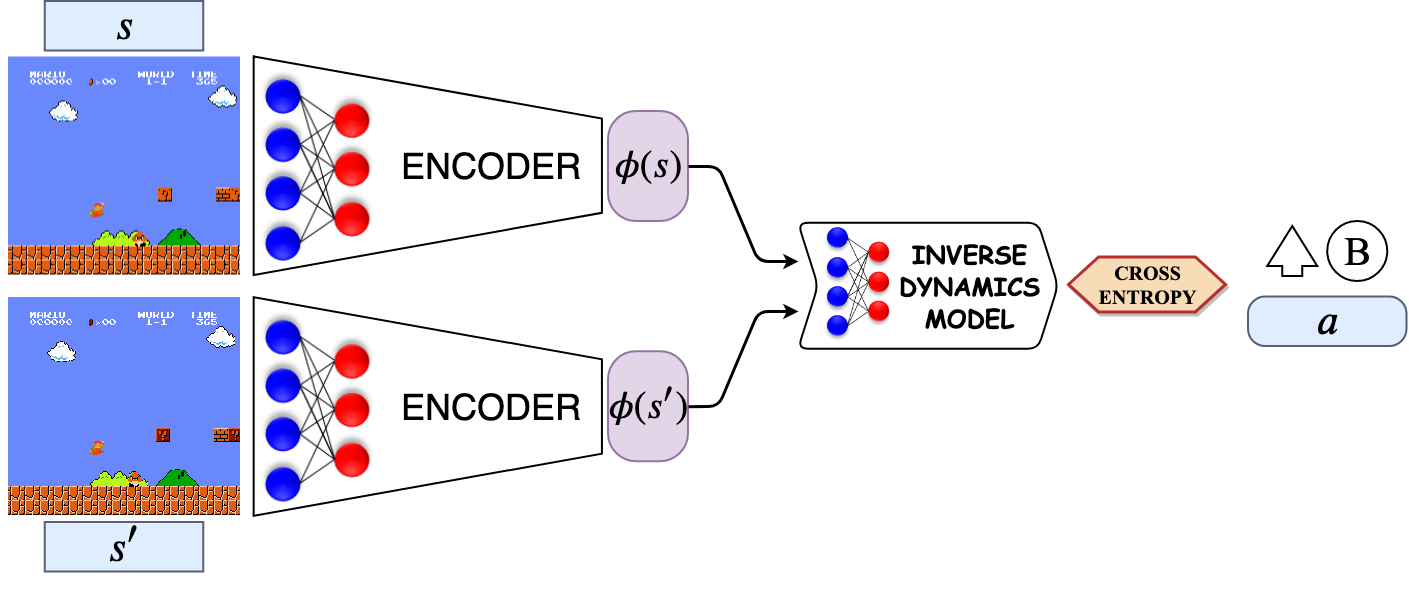
\includegraphics[width=0.5\textwidth]{Images/inversemodel.png}
\vspace{-0.7cm}
\end{wrapfigure}

В ICM предлагается починить проблему шумных телевизоров следующим образом. Строится модель обратной динамики с <<сиамской>> архитектурой; для непрерывных пространств действий задача выглядит так:
$$\E_{s, a, s'} \|g(\phi(s), \phi(s')) - a\|^2_2 \to \min_{g, \phi},$$
а для классификации как
$$\E_{s, a, s'} \log g(a \mid \phi(s), \phi(s')) \to \max_{g, \phi},$$
где $\phi(s) \colon \St \to \R^d$ строит некоторое латентное описание состояний --- фильтр, --- а затем функция $g$ пытается восстановить действие $a$, случившиеся между двумя состояниями, по их латентным описаниям. Тогда функция $\phi$ будет оставлять от состояний только информацию, необходимую для предсказания промежуточных действий. Скорее всего, эта информация будет соответствовать описанию только тех объектов в среде, с которыми агент может непосредственно провзаимодействовать, по изменению состояний которых можно судить о том, какое действие совершил агент. Таким образом, $\phi(s)$ будет выдавать \emph{контролируемое состояние} (controlable state), очищенное от нерелевантных для агента явлений.

Основная идея ICM заключается в том, что модель прямой динамики должна строиться в таком <<отфильтрованном>> латентном представлении:
\begin{equation}\label{ICMforward}
\E_{s, a, s'} \|f(\phi(s), a) - \phi(s')\|^2_2 \to \min_{f}
\end{equation}

Авторы предложили обе модели обучать совместно, то есть в частности оптимизировать \eqref{ICMforward} по параметрам фильтра $\phi$. Итого модель ICM выглядит следующим образом:
$$\E_{s, a, s'} \left[ \|g(\phi(s), \phi(s')) - a\|^2_2 + \alpha \|f(\phi(s), a) - \phi(s')\|^2_2 \right] \to \min_{f, g, \phi}$$
где $s, a, s'$ --- произвольные тройки из любого буфера, $\alpha$ --- масштабирующий гиперпараметр. 

\needspace{10\baselineskip}
\begin{wrapfigure}{r}{0.5\textwidth}
\vspace{-0.4cm}
\centering
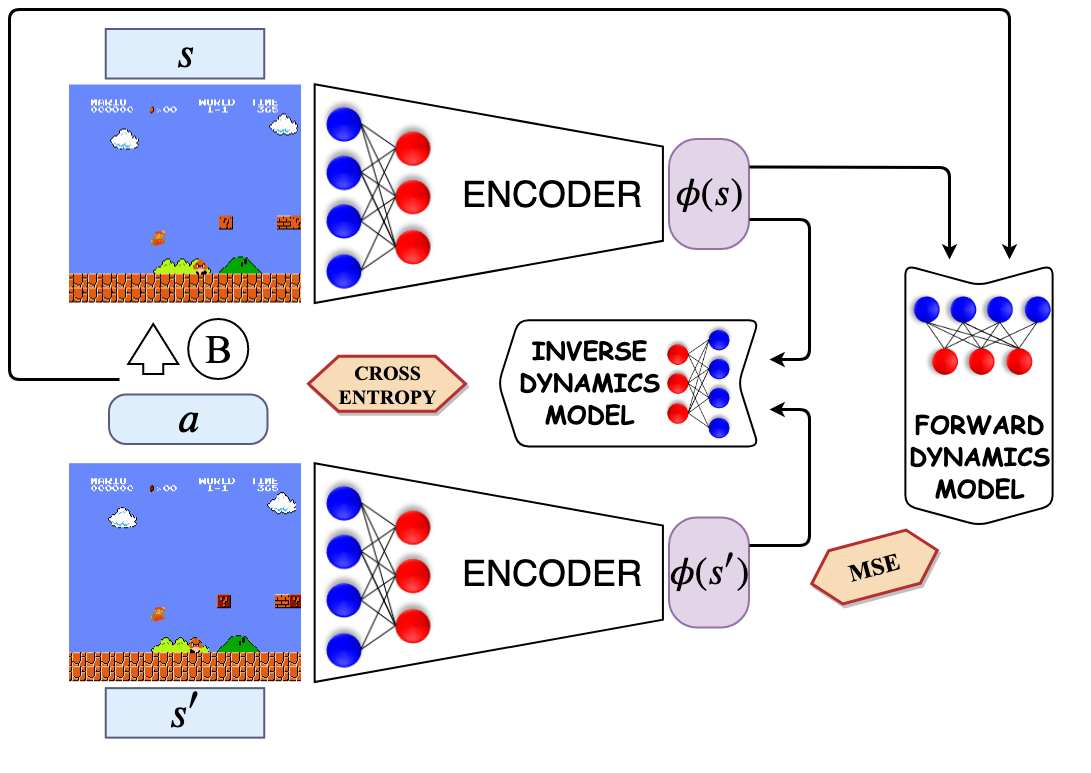
\includegraphics[width=0.5\textwidth]{Images/ICM.png}
\vspace{-0.5cm}
\end{wrapfigure}

В этой задаче оптимизации градиенты нигде не останавливаются: это значит, что от фильтра $\phi$ требуется построение таких представлений, в рамках которых модели прямой динамики $f$ <<проще всего>> предсказывать будущее. Понятно, что, если бы первого слагаемого (задачи обратной динамики) в таком функционале не было бы, оптимальным решением было бы $\phi(s) \HM= \const$. Можно считать, что модель прямой динамики выступает регуляризатором для модели обратной динамики: представления $\phi(s)$ одновременно должны содержать достаточно информации для предсказания выбранных действий и при этом быть максимально простыми.
%Аналогичная задача для дискретных пространств действий строится заменой в модели обратной динамики регрессии на классификацию:
%$$\E_{s, a, s'} \left[-\log g(a \mid \phi(s), \phi(s')) + \alpha \|f(\phi(s), a) - \phi(s')\|^2_2 \right] \to \min_{f, g, \phi}$$

В качестве внутренней мотивации используется только ошибка модели прямой динамики:
\begin{equation*}
r^{\intr}(s, a, s') \coloneqq \|f(\phi(s), a) - \phi(s')\|^2_2
\end{equation*}

Решает ли ICM проблему шумных телевизоров? Теоретически, можно рассчитывать на то, что модель обратной динамики отфильтрует те шумные телевизоры, с которыми агент не может провзаимодействовать. Но если у агента есть <<пульт>> от телевизора, если случайное непредсказуемое явление можно <<затриггерить>> определёнными действиями, то ICM всё равно приведёт к прокрастинации.

\begin{exampleBox}[label=ex:controltv]{Управляемый шумный телевизор}
В среде присутствует телевизор, демонстрирующий изображение (возможно, осмысленное!) из разнообразного бесконечного набора. У агента есть пульт от телевизора, то есть действие $\hat{a}$, при выборе которого изображение на телевизоре сменяется на случайное из набора. По факту смены изображения между $s$ в $s'$ модель обратной динамики может сделать однозначный вывод о том, что между состояниями было выбрано именно действие $\hat{a}$, следовательно в представлении $\phi(s)$ останется информация о содержимом телевизора. При этом, в силу случайности выбора изображения из набора, предсказать контент телевизора по предыдущему изображению и факту нажатия на пульт невозможно. Следовательно, модель прямой динамики в ICM будет ошибаться на тройках, содержащих $\hat{a}$, и агент будет мотивирован бесконечно выбирать действие $\hat{a}$.
\end{exampleBox}

% \begin{wrapfigure}{L}{0.25\textwidth}
% \centering
% \includegraphics[width=0.2\textwidth]{remotecontrol}
% \caption{\label{fig:remotecontrol}Пример управляемого шумного телевизора: у агента есть пульт, рисующий случайные <<круги>> на стенах лабиринта, никак не связанные с задачей.~\citep{savinov2018episodic}}
% \end{wrapfigure}

Шумные телевизоры, с которыми агент может провзаимодействовать, представляют собой любые стохастичные явления в среде, которые агент может <<запускать>> своими действиями. Это не столько проблемой самого алгоритма ICM, сколько концептуальная проблема любопытства. Наличие у агента возможности взаимодействовать с шумным телевизором потенциально означает, что некоторая комбинация действий приводит к решению искомой задачи в среде (высокой внешней награде), а сам шумный телевизор --- связан с задачей (в примере \ref{ex:controltv} с управляемым шумным телевизором задача гипотетически могла заключаться в поиске определённого изображения из набора, или совершении определённой комбинации действий при определённых условиях на текущее отображаемое изображение). При этом любопытство, как и любая внутренняя мотивация, вводится из соображений, что априорных знаний об истинной задаче агента не дано, и произвольные явления в среде должны быть исследованы.

\begin{remark}
В большинстве традиционных задач для тестирования алгоритмов RL такие управляемые телевизоры обычно отсутствуют; обычно, для того, чтобы <<сломать>> ICM, нужно строить специальную среду. 
\end{remark}

% \subsection{Эпизодичное исследование}

% Затухание внутренней мотивации приводит к тому, что агент может перестать заходить в некоторые области. Чтобы гарантировать

% Never Give Up дополнительно ввёл эпизодичную награду за посещение состояний, которые ещё не встречались в течение данного эпизода. Состояния переводятся в эмбеддинги при помощи фильтра $\phi(s)$ из модели обратной динамики для получения описания <<контролируемого состояния>> (controllable state). Эмбеддинги всех встречавшихся за эпизод состояний складываются в буфер $M$. На очередном шаге эмбеддинг очередного состояния $q$ сравнивается со всеми описаниями $k \in M$ и высчитывается <<эпизодичная>> награда на данном шаге:
% $$r^{\mathrm{episodic}} \coloneqq \frac{1}{\sqrt{\sum_{k \in N_k} \rho(q, k)} + c}$$
% где $N_k$ --- $k$ ближайших соседей $q$ из $M$, $c$ --- маленькая константа, и
% $$\rho(q, k) = \frac{\epsilon}{\epsilon + \frac{\|k - q\|^2_2}{d}},$$
% где $d$ --- бегущее среднее величины $\sum_{k \in N_k} \rho(q, k)$.

% Эта награда совмещается с наградой $r^{\mathrm{RND}}$ из RND следующим образом:
% $$r_{\intr} \coloneqq r^{\mathrm{episodic}} \operatorname{clip}(r^{\mathrm{RND}}, 1, L),$$
% где $L$ --- константа.

% TODO: интуиция формулы ядра (счётчики) и RND на самом деле $1 + \frac{r - m}{\sigma}$.